\section{Proposed Method} 
In chapter 1, we learned a generative model of gene expression time
series data using a VAE framework, where we learned a regularized latent space representation of latent
variables $z$ by reconstructing the data $x$ through an encoder-decoder architecture. We can start
thinking about the binding element design problem in the same manner.

Let's define $x_p$ as input binding site information. We want to predict a binding element $x_e$
given $x_p$. To achieve this task, we again formulate a generative story: $x_e$ is generated from
latent variables $z$, which can be modeled by a decoder/generator network which models the
distribution $P(x_e|z)$. And we can employ an encoder network modeling $P(z|x_p)$ to achieve the
latent information $z$ from the input $x_e$.

Now, to formally achieve the prediction task, we start with writing out the conditional distribution,
$P(x_e, z|x_p)$ which we would like to maximize and predict the argument $x_e$ and $z$ that maximizes it.

\begin{align*}
        P(x_e,z|x_p) = P(x_e|z,x_p)P(z|x_p) \;\;\; \text{using conditional probability  rule}\numberthis
\end{align*}
Here, we assume a hierarchical Bayesian setting where given the latent variable $z$, $x_e$ is
generated independent of $x_p$ i.e. $P(x_e|z,x_p) = P(x_e|z)$. Now we can write the following,
\begin{align*}
P(x_e,z|x_p) &= P(x_e|z)P(z|x_p) \numberthis \\
\end{align*}
Now, we can model the posterior of $z$, $P(z | x_p)$ as a Gaussian $N(z_{\mu}, z_{\Sigma})$ where $z_{\Sigma}$ is diagonal. This
can be modeled by outputting the parameters $z_{\mu}, z_{\Sigma}$ from an encoder network $E(x_p)$.
A value of $z$ can be sampled from this distribution now using the reparametrization trick described
in \citet{Kingma2014}, similar to as described in Chapter 1 for RVAgene. This process along with a
KL loss with a prior on $z$, $p(z) = N(0,\bI)$ ensures a regularized latent space which is important
for generating meaningful data. Therefore,
\begin{align*}
        z_{\mu}, z_{\Sigma} &= E(x_p) \numberthis \\
        \hat{z} &= z_{\mu} + \epsilon \cdot z_{\Sigma} \;\; where \;\; \epsilon \sim \cN(0,\bI) \numberthis \\
        \hat{x}_e &= argmax_{x_e}p(x_e | \hat{z}) = G(\hat{z}) \;\; \numberthis \label{final_prediction_architecture} 
\end{align*}
%\implies \text{prediction } \hat{x}_e, \hat{z} &= argmax_{x_e,z} P(x_e,z|x_p) \numberthis \\
%&= argmax_{x_e,z} P(x_e|z)P(z|x_p)  \\
%\implies  \hat{z} = argmax_{z} P(z|x_p); & \;\;\;\;\hat{x}_e = argmax_{x_e} P(x_e | \hat{z}) \numberthis \\
%\implies \hat{z} = E(x_p); & \;\;\;\; \hat{x}_e = G(\hat{z}) \numberthis
The functions $E(x_p)$ and $G(\hat{z})$ in \ref{final_prediction_architecture} represent the
encoder and generator functions respectively both of which are parametrized by neural networks. 
\hyperref[fig:design]{Fig. 3.2} schematically describes the model details described in this section.
The exact architecture of Encoder $E$ and Generator $G$ shown in \hyperref[fig:design]{Fig. 3.2}
is not decided and will vary for the drug molecule generation setting from the nucleic acid PWM
generation setting.
Now, we need to think about how to train this model, in case of RVAgene the input and output to the
model was the same: gene expression time-series data, and we could employ a reconstruction loss to
give the model an objective to optimize. Here, we can do something similar. We shall have the same
KL divergence loss as we had for RVAgene, and we shall have a prediction loss comparing generated
$\hat{x}_e$ to true $x_e$. However, this term won't be as straightforward as a reconstruction loss
always. The following equation described the training objective of the model:
\begin{align*}
        \cL(\theta, x_e) = D_{KL}(\cN(z_{\mu},z_{\Sigma}) || \cN(0,\bI)) + f(x_e, \hat{x}_e)
        \numberthis \label{loss}
\end{align*}
The definition of the prediction loss $f(x_e, \hat{x}_e)$ will change depending on the
representation and type of binding element begin generated. For sequence PWMs it will be a
straightforward L1($|x_e -  \hat{x}_e|$) or L2 loss ($|x_e -  \hat{x}_e|^2$). For SMILES strings, it
can be L1/L2 loss on the one hot encodings of the SMILES strings or it can also be some kind of
sequence alignment based scoring scheme. For molecular graph representations some for graph
similarity/distance measurement can be used to implement $f$. It can be a straightforward L1/L2 loss
between the vertex/edge features and adjacency matrices of $x_e$ and $\hat{x}_e$. Otherwise, we can
use some more involved approaches detailed in \citet{koutra2011algorithms} or more recent approaches
like \citet{lin2019novel}. Once we have decided  $f$, the whole model can be trained by the standard
backpropagation \citep{kelley1960gradient} algorithm for neural network training using the loss
function described in \ref{loss}.
\begin{center}\begin{figure}
                \makebox[\textwidth]{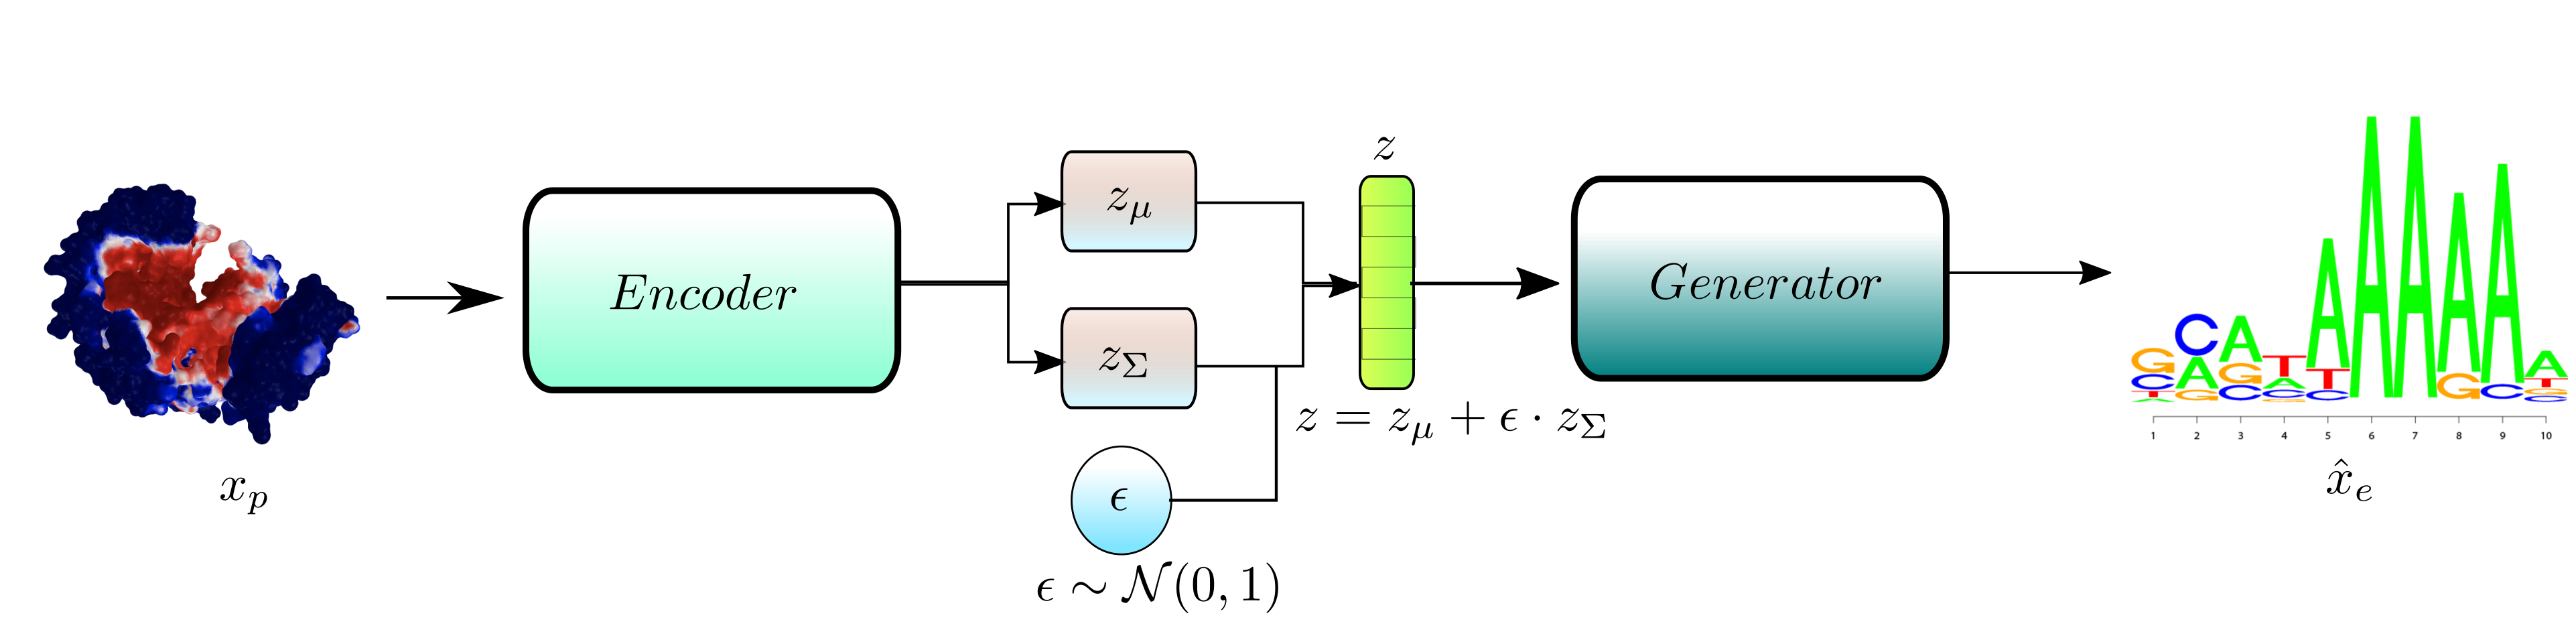
\includegraphics[width=0.8\paperwidth]{design_figs/design.png}}
 % archetecture.png: 1149x508 px, 72dpi, 40.53x17.92 cm, bb=0 0 1149 508
        \caption[Proposed model for binding element design]{\textbf{Proposed model for binding element design}}
        \label{fig:design} \end{figure} \end{center}
%Now, the encoder-generator framework described above is suitable for prediction, however it's
%difficult to train it in a straight forward manner. For RVAgene \red{(cite)} we were able to use
%reconstruction based method to train because the input of encoder and output of decoder was the same.
%Here, they are different. This constitutes a proper scenario to employ an adversarial training
%scheme as employed by GANs \citep{goodfellow2014generative}.
%
%Given a training dataset $X$ consisting of $n$ datapoints, where $X_i = (x_p^i, x_e^i) \;\; i \in
%\{0,..., n-1\}$, we now describe
%how to train the generative model described in \ref{final_prediction_architecture}. We assign a
%label variable $y = 1$ for all datatpoints in the training data $X$. Now, assume we have some
%datapairs $F = (x_p^i, \hat{x}_e^i) \;\; i \in \{0,..., m-1\}$ generated by the encoder-generator
%system given $x_p^i$s as input. We assign these datapoints a label $y = 0$. Now, we can train a
%neural network $D$ discriminating between the datasets X and F i.e. the discriminator $D$ is
%predicting $P(y = 1 | x_p, x_e)$. It is clear that the better the enocder-generator system is in
%predicting binding element given a protein surface, the harder the job of the discriminator becomes.
%We take advantage of this fact and teach the encoder-generator network to try to best the
%discriminator and vice versa. The two networks play the following minimax game:
%\begin{align*}
%        min_{G,E}max_{D} V(D, E, G) &= \bE_{x_p, x_e \sim P_X}\bigg{[}log D(x_p, x_e)\bigg{]} + \bE_{x_p \sim
%        P_{x_p}}\bigg{[}log(1 - D(x_p,G(\hat{z}))) + KL(N(z_{\mu}, z_{\Sigma}) || N(0, \bI))\bigg{]} \numberthis \label{gan_game}\\
%        &where \; \hat{z} = z_{\mu} + \epsilon z_{\Sigma} \;\; where \; \epsilon \sim N(0,\bI)\; and \;
%        z_{\mu}, z_{\sigma} = E(x_p)
%\end{align*}
%In eq. \ref{gan_game} above $P_X$ represents the full training data distribution and $P_{x_p}$
%represents the marginal distribution of binding sites in the training data. 
%
%If we call the generated distribution of $x_p, \hat{x}_e$ as $p_g$, as described and proven in
%\citet{goodfellow2014generative} this adversarial game 
%eventually results into the generated data distribution becoming same as the training data
%distribution $P_x$, which
%happens at the point when both the $(E, G)$ and $D$ network cannot improve anymore.
%
%Algorithm \ref{algo:GAN_training} describes the training algorithm odddf the model described above.
%\begin{pmialgorithm}[0.9\textwidth]{h!}{CCRF Layer}\vskip-2ex
%        \label{algo:GAN_training}
%        \begin{algorithmic}[1]
%                \REQUIRE  $X = (x_p^i, x_e^i) \; \forall \; i \; \in \; \{0,..., n-1\}$
%                \FOR{number of training itrations}
%                    \STATE sample minibatch of m training datapoints
%                \ENDFOR
%                \STATE Initialize $H_i^0 = B_i$ $\forall i$\COMMENT{$H_i^0$ maximises $Q_i^0 = \frac{1}{Z_i^0}exp(-c||H_i^0 - B_i||^2)$}
%                \FOR[$T$ signifies convergence]{$t=0,1,2,...,T-1$}
%        \STATE compute $(\sum \limits_{j \in \mathcal{N}(i)} (g_{ij} H_j^t),\sum \limits_{j \in \mathcal{N}(i)} g_{ij})$ \COMMENT{message passing}
%        \STATE $H_i^{t'} = \alpha B_{i} + \beta  \sum\limits_{j \in \mathcal{N}(i)} (g_{ij} H_j^t)$
%        \STATE $H_i^{t+1} = H_i^{t'} / (\alpha +  \beta  \sum \limits_{j \in \mathcal{N}(i)} g_{ij} )$
%                \ENDFOR
%                \STATE $H_i^* = H_i^T$
%                \RETURN $H_i^*$
%        \end{algorithmic}
%\end{pmialgorithm}


